\chapter{Motion Planning and Control}

\section{Exercise 1 - route planning}

\textbf{Q. Optimize the route planning task using RRT* algorithm}

The optimization included multiple parameters which are listed below along with the values tested for each one:

\begin{itemize}
    \item \textbf{connection distance (c\_dist):} decides the maximum distance allowed when sampling for a new vertex. Generated vertices are closer together with shorter distance. \newline [20, 30, 35, 40, 45, 50, 55, 60 , 70] m
    \item \textbf{number of iterations (itr):} how many times to generate new vertices. Number of generated vertices increase with higher iterations. \newline
    [($10^{2} \rightarrow 10^{3}$), ($10^{3} \rightarrow 10^{4}$), ($10^{4} \rightarrow 10^{5}$), ($10^{5} \rightarrow 10^{6}$)]
    \item \textbf{max allowable steering angle ($\delta$):} decides the maximum angle the vehicle can steer.\newline
    [4, 5, 6, 7, 8] $^\circ$
    \item \textbf{interpolation samples:} the space between vertices to sample from. The smaller the number the bigger the sampling pool. \newline
    [10, 30, 50, 70, 90]
\end{itemize}

The optimization metrics are mainly the elapsed time taken to calculate the distance of the generated path, and the smoothness of said path.

Figure \ref{71eltm} and Table \ref{tab:7.1} show the time taken for the RRT* to calculate the reference path. The results are categorized based on two variables, the connection distance and the number of iterations of the algorithm.

       \begin{figure}[ht]
        \includegraphics[width=0.7\linewidth]{ex7/q1/ex-71eltm.eps}
        \centering
        \caption{combined effect of c\_dist and iteration count on elapsed calculation time}
        \label{71eltm}
        \end{figure}

It appears that there is no co-relation between the connection distance and elapsed time. The biggest impacting variable on elapsed time is the number of iterations. Going from minimum iteration of $10^{4}$ to $10^{5}$ increased the elapsed time by 20 folds.

\begin{table}[ht]
    \centering
    \begin{tabular}{c | c | c | c | c}
      \textbf{c\_dist [m]}  & \textbf{itr =$10^{2}$} & \textbf{itr =$10^{3}$} & \textbf{itr =$10^{4}$} & \textbf{itr =$10^{5}$} \\ \hline
      20 &  0.4 s &  0.2 s  &  1.3 s &  20.8 s    \\\hline
      35 &  .1 s &  .1 s  &  1.2 s &  18.1 s \\\hline
      45 &  NA &  .1 s  &  1.2 s &  18.6 s \\\hline
      55 &  .1 s &  .1 s  &  1.2 s &  20.8 s \\\hline
      70 &  NA  &  .1 s  &  1.1 s &  21.4 s \\
    \end{tabular}
    \caption{elapsed time results for connection distance and iteration count]}
    \label{tab:7.1}
\end{table}

The resulting paths from RRT* are plotted in Figure \ref{71cds} and \ref{71itr} to further analyse the effect of connection distance and iteration count. 
       \begin{figure}[ht]
        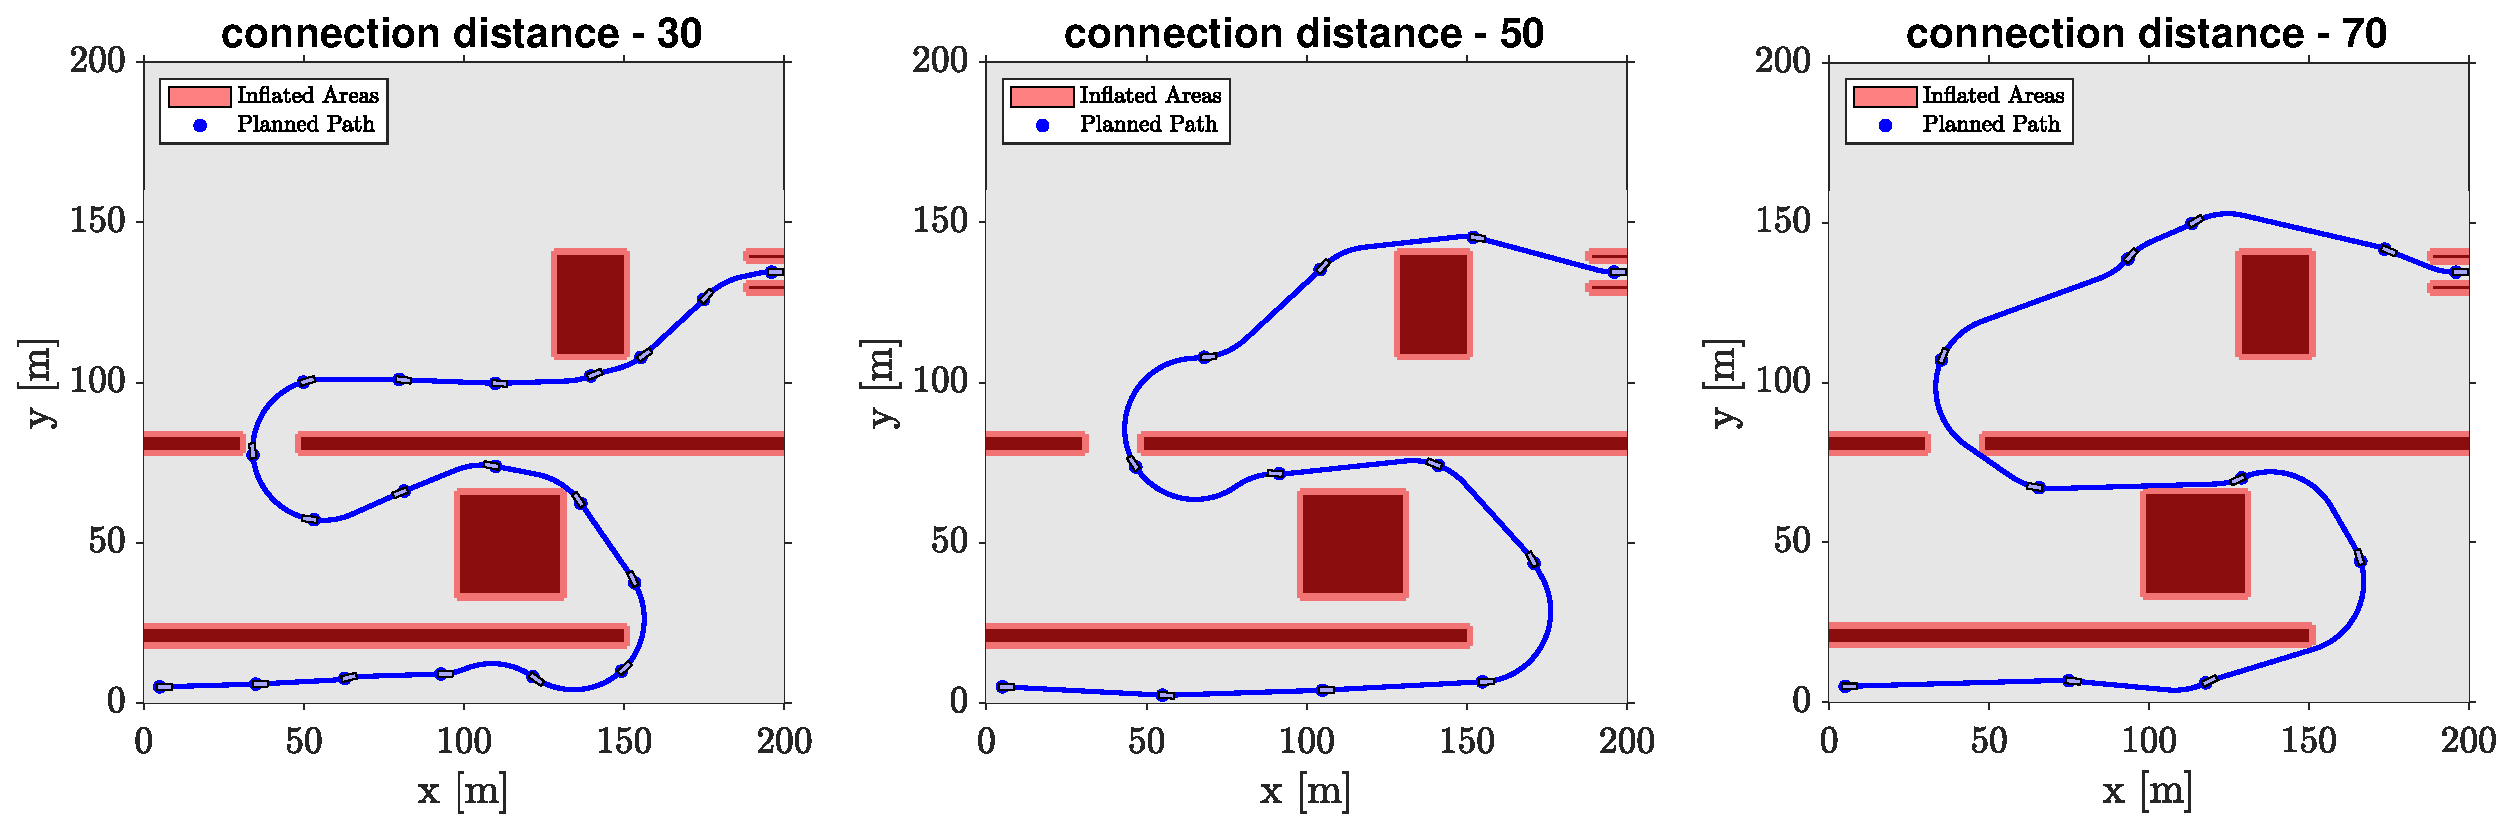
\includegraphics[width=0.99\linewidth]{ex7/q1/ex-71cds.eps}
        \centering
        \caption{connection distance effect on RRT* [min itr =$10^{5}$]}
        \label{71cds}
        \end{figure}
        
The smaller the connection distance, the closer the vertices on the path. When the distance between vertices are smaller the path appear to have more turns and more steering input. 

Decreasing the distance has no major impact from a computational time prospective. However, it could negatively impact the controller's capability of tracking the reference path. As shown in Figure \ref{71cdis3}, with smaller connection distance, the tracking error increases.

       \begin{figure}[ht]
        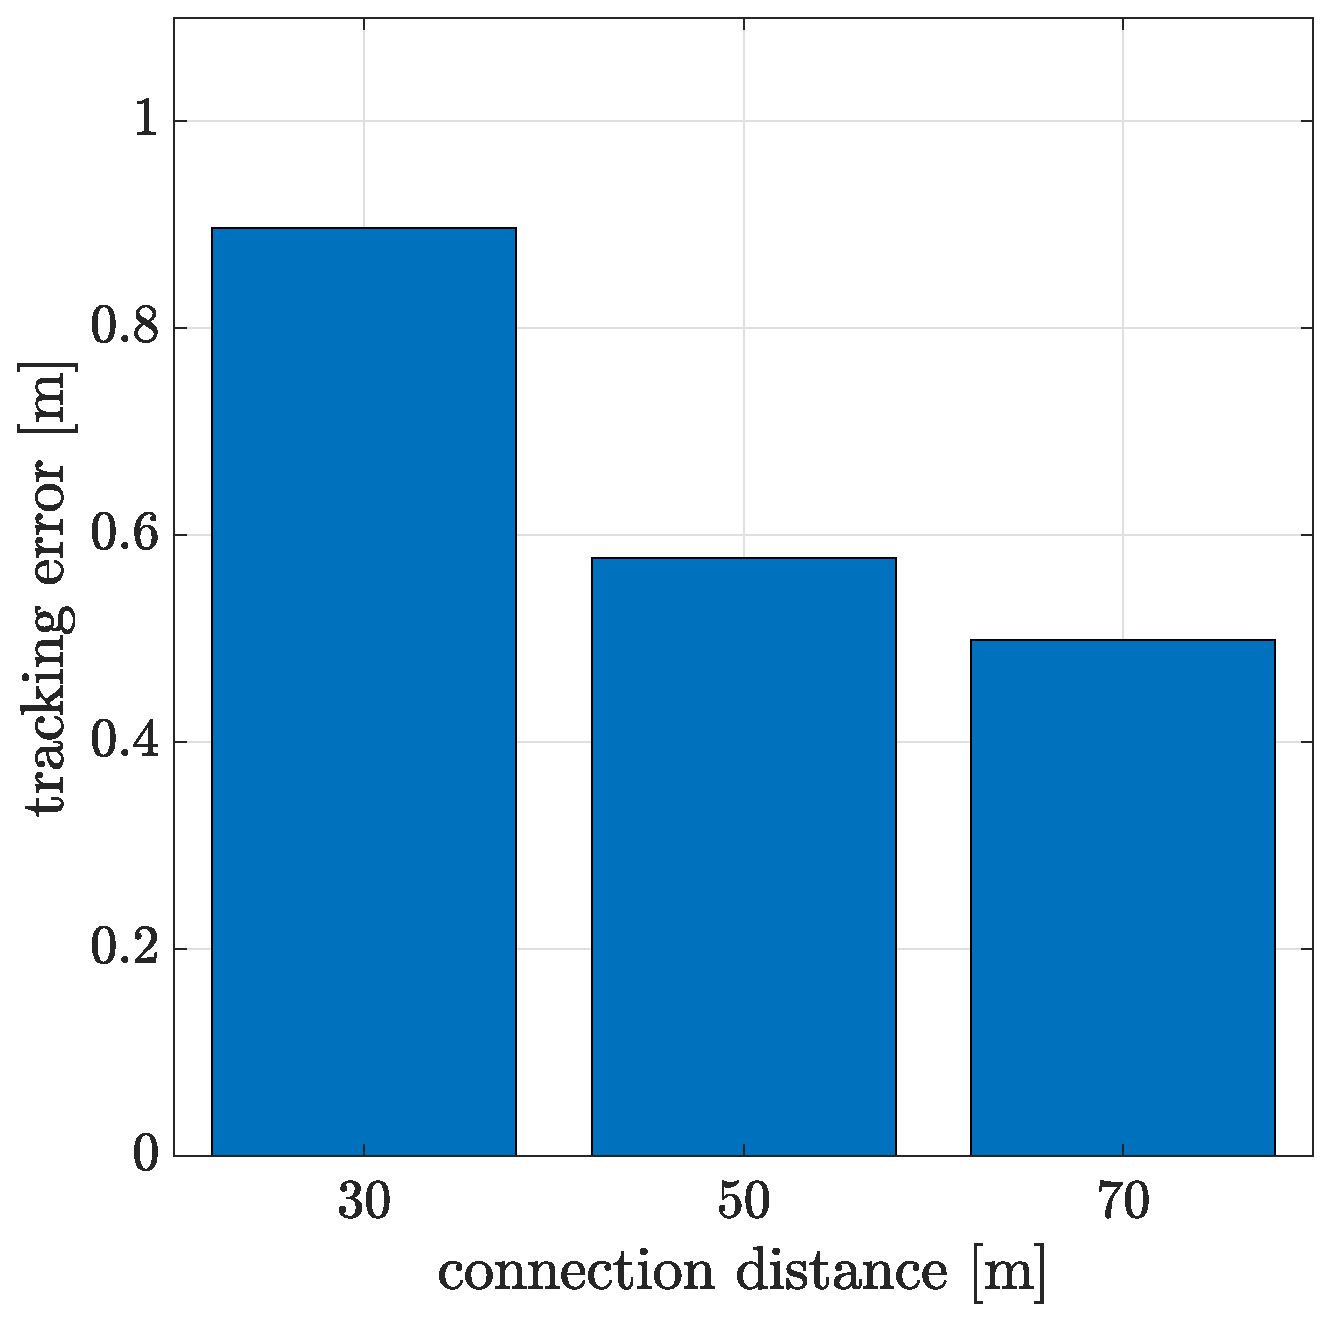
\includegraphics[width=0.54\linewidth]{ex7/q1/ex-71cdis3.eps}
        \centering
        \caption{Tracking error at 50km/h with different connection distances}
        \label{71cdis3}
        \end{figure}
        
Figure \ref{71itr} shows that increasing the iteration count improves the path optimization. Higher iteration count allows RRT* to find a better solution that has a smaller distance. The average distance of the total path for each iteration count was calculated based on 30 different tests and the results are shown in Figure \ref{71rl}. 

       \begin{figure}[ht]
        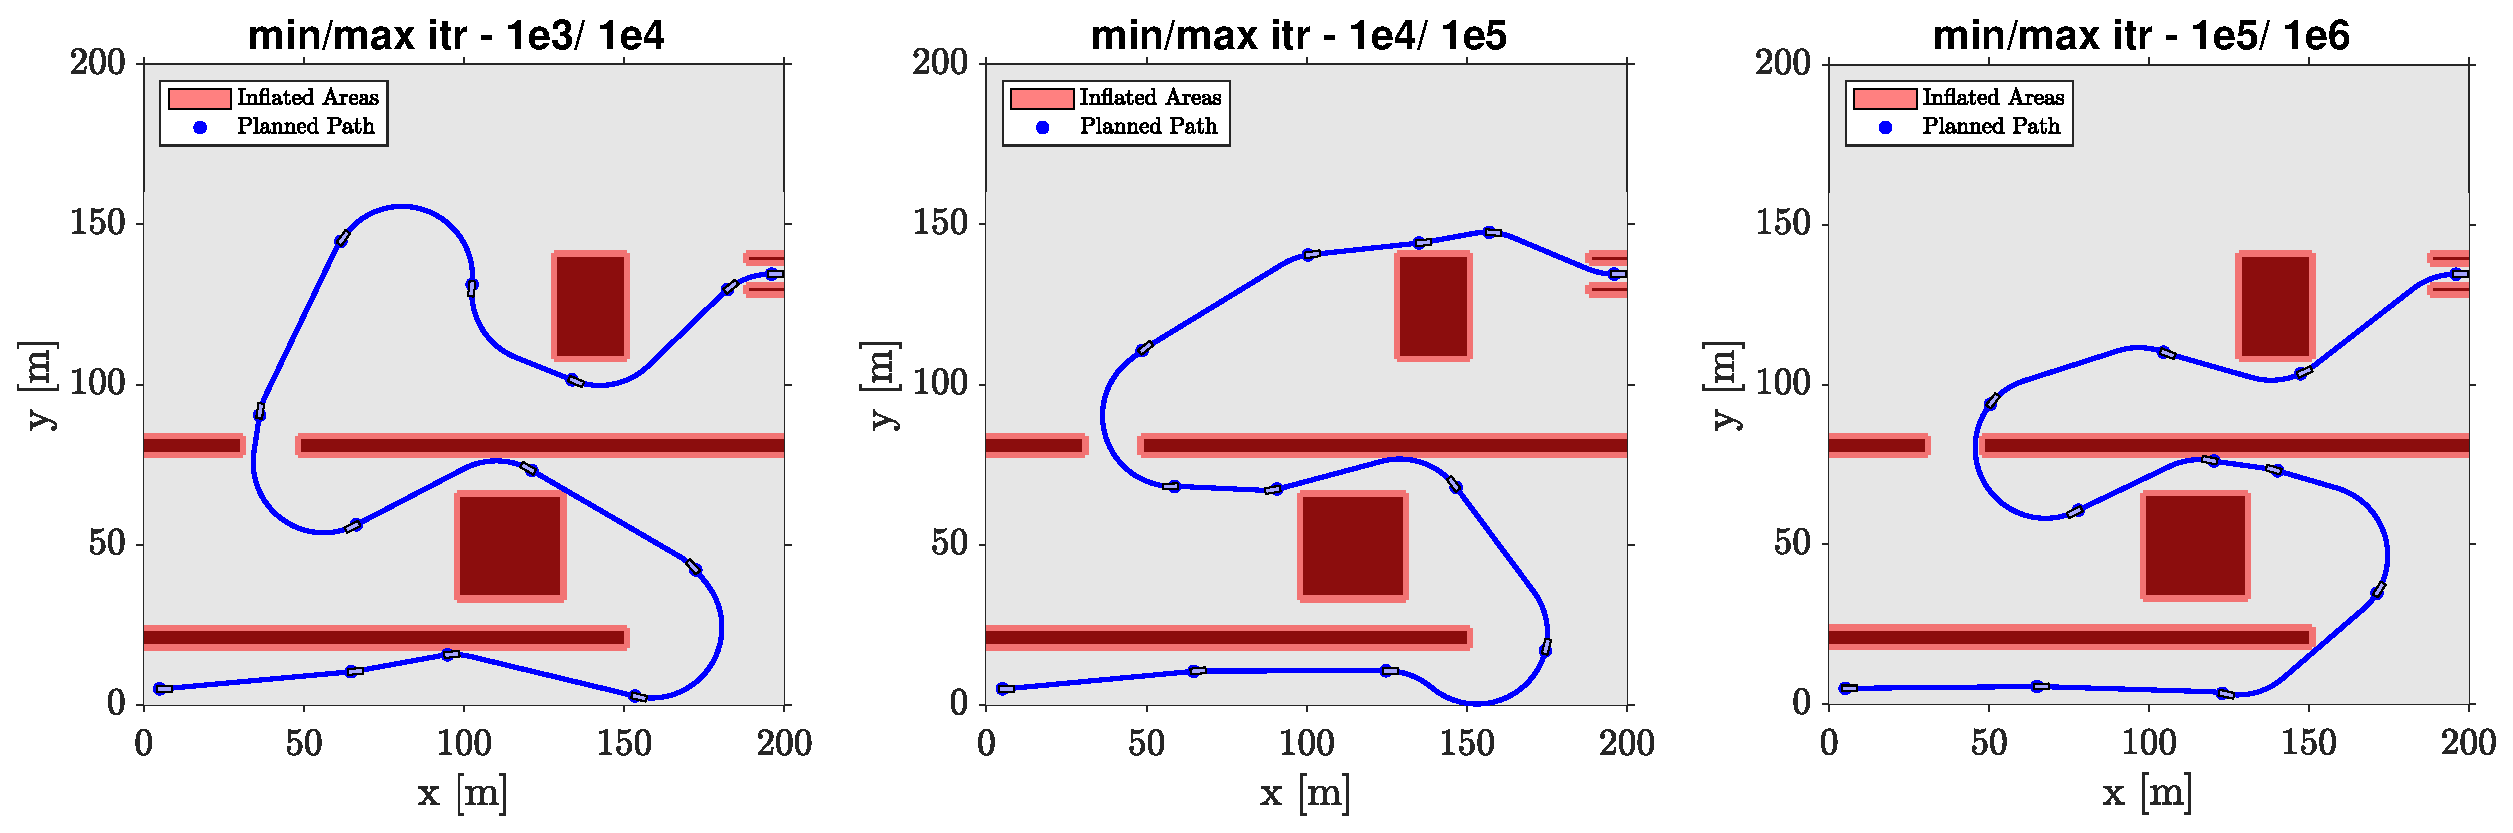
\includegraphics[width=0.99\linewidth]{ex7/q1/ex-71itr.eps}
        \centering
        \caption{number of iterations effect on RRT* [connection distance = 60]}
        \label{71itr}
        \end{figure}

The percent improvement achieved going from minimum iteration of $10^{4}$ to $10^{5}$ is only 2\% [533 $\rightarrow$ 524 m]. This was not quite worth it as the elapsed time taken to compute increased 20 times. Therefore, the best minimum/maximum iteration count is $10^{4} \rightarrow 10^{5}$.

       \begin{figure}[ht]
        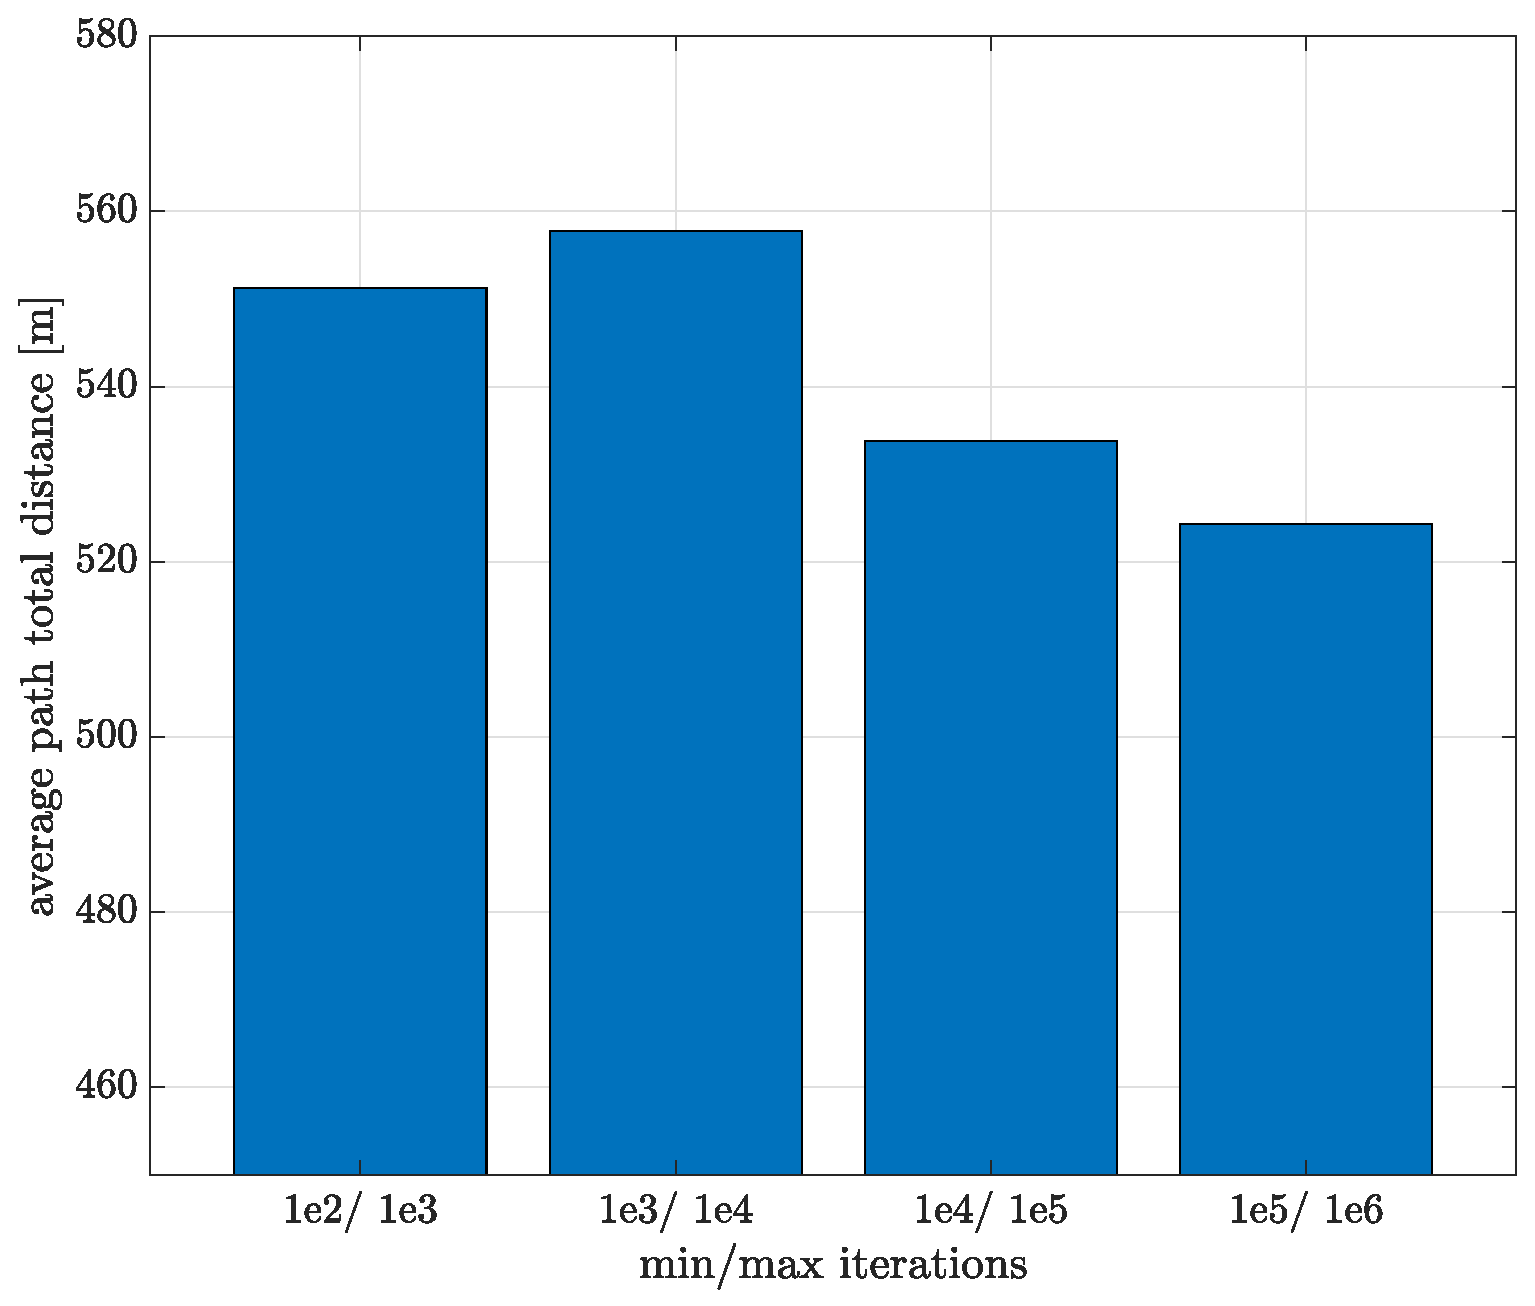
\includegraphics[width=0.6\linewidth]{ex7/q1/ex-71rl.eps}
        \centering
        \caption{Generated path average total distance for each iteration count}
        \label{71rl}
        \end{figure}

The effect of maximum steering angle $\delta$ would impact the dynamics of the vehicle much more than RRT*. That is why Figure \ref{71mst2} shows the generated path along with the real tracked path using the clothoid lateral controller optimized previously. The biggest difference in the RRT* generated path is that the radius of curvature can be smaller with larger $\delta$, which in theory should increase the chances of finding a feasible solution.

       \begin{figure}[ht]
        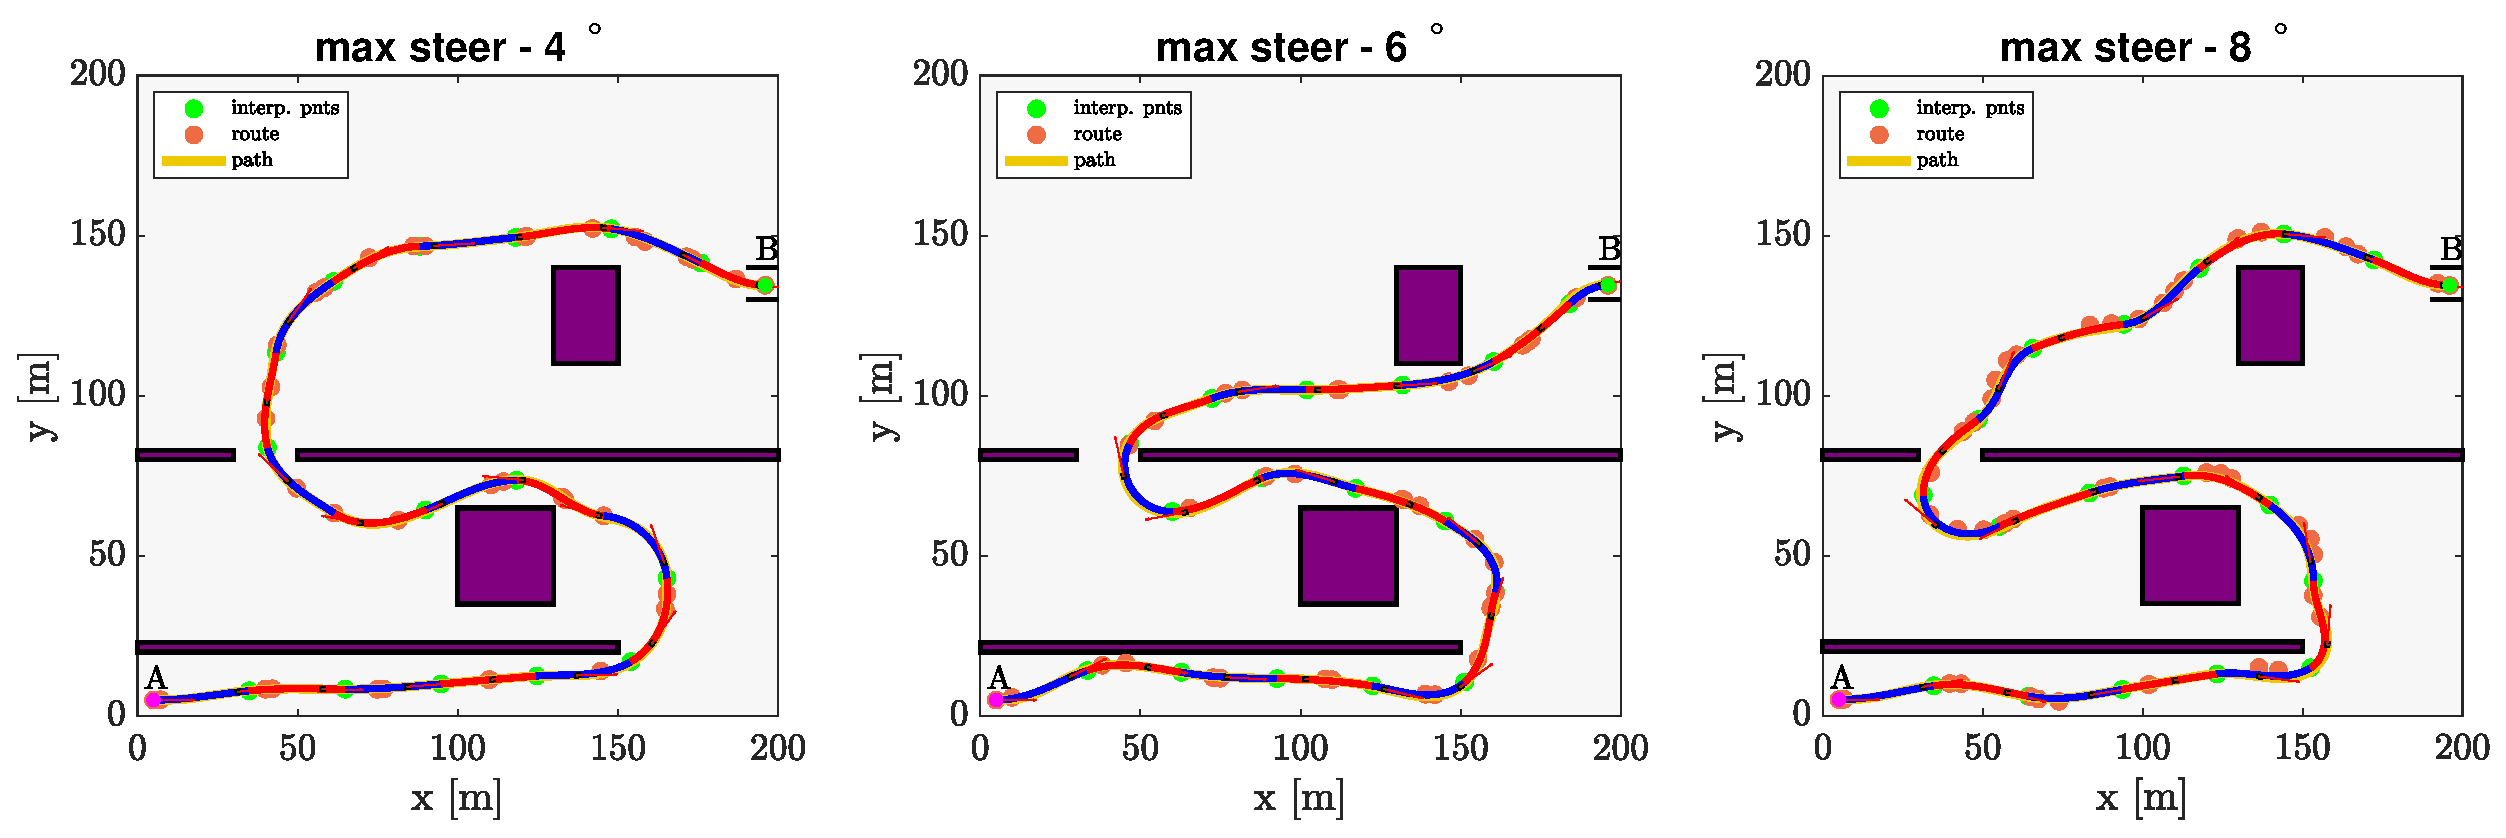
\includegraphics[width=0.99\linewidth]{ex7/q1/ex-71mst2.eps}
        \centering
        \caption{max $\delta$ effect on RRT* and path tracking at 50km/h [min itr =$10^{5}$]}
        \label{71mst2}
        \end{figure}
        
Tracking becomes more difficult with increasing $\delta$, especially with higher speeds. In Figure \ref{71mst3}, the tracking error was calculated for each steering angle with a velocity $u$ = 50 km/h. A max steering angle of 5$^\circ$ is preferred.
        \begin{figure}[ht!]
        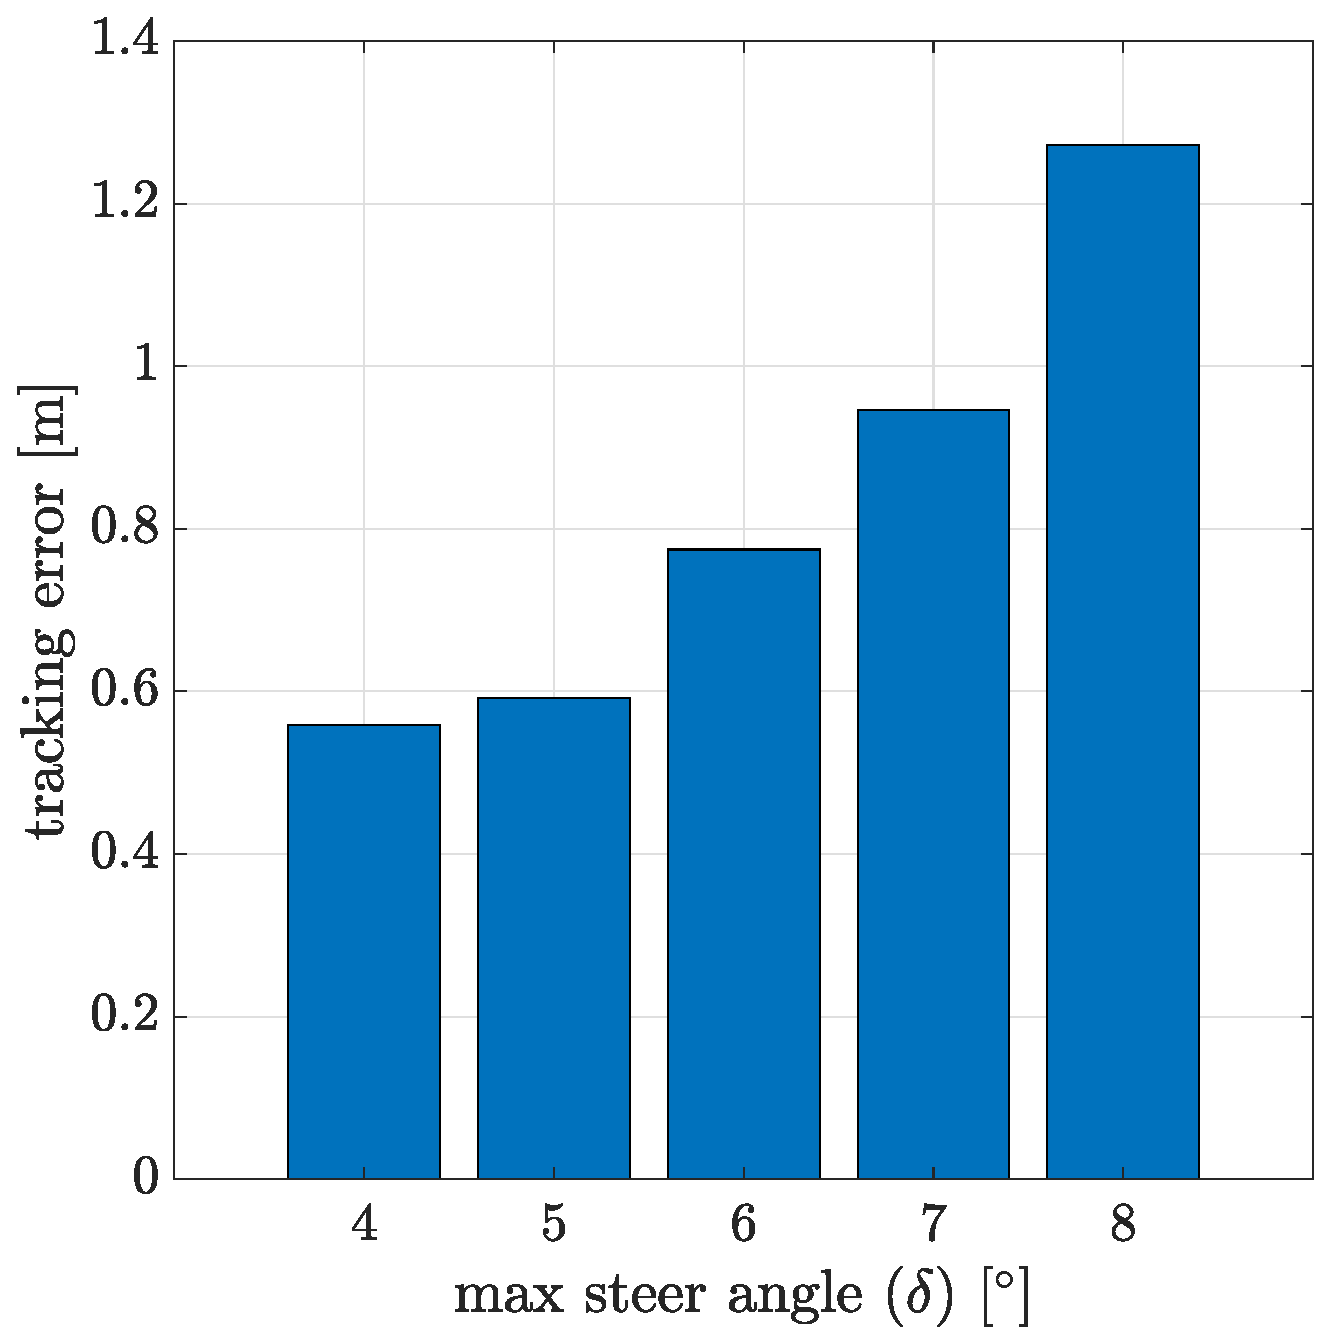
\includegraphics[width=0.6\linewidth]{ex7/q1/ex-71mst3.eps}
        \centering
        \caption{Tracking error at 50 km/h with different max $\delta$}
        \label{71mst3}
        \end{figure}
    
The interpolation samples parameter was tested on the same generated route to examine its effect. A route was generated using [c\_dist = 35, itr = $10^{4}$, $\delta$ = 5$^\circ$]. The path was then interpolated with five different numbers in which three of them are shown in Figure \ref{71samp1}. The resolution of the path [number of vertices] decreases with an increase in the interpolation sample.

        \begin{figure}[ht]
        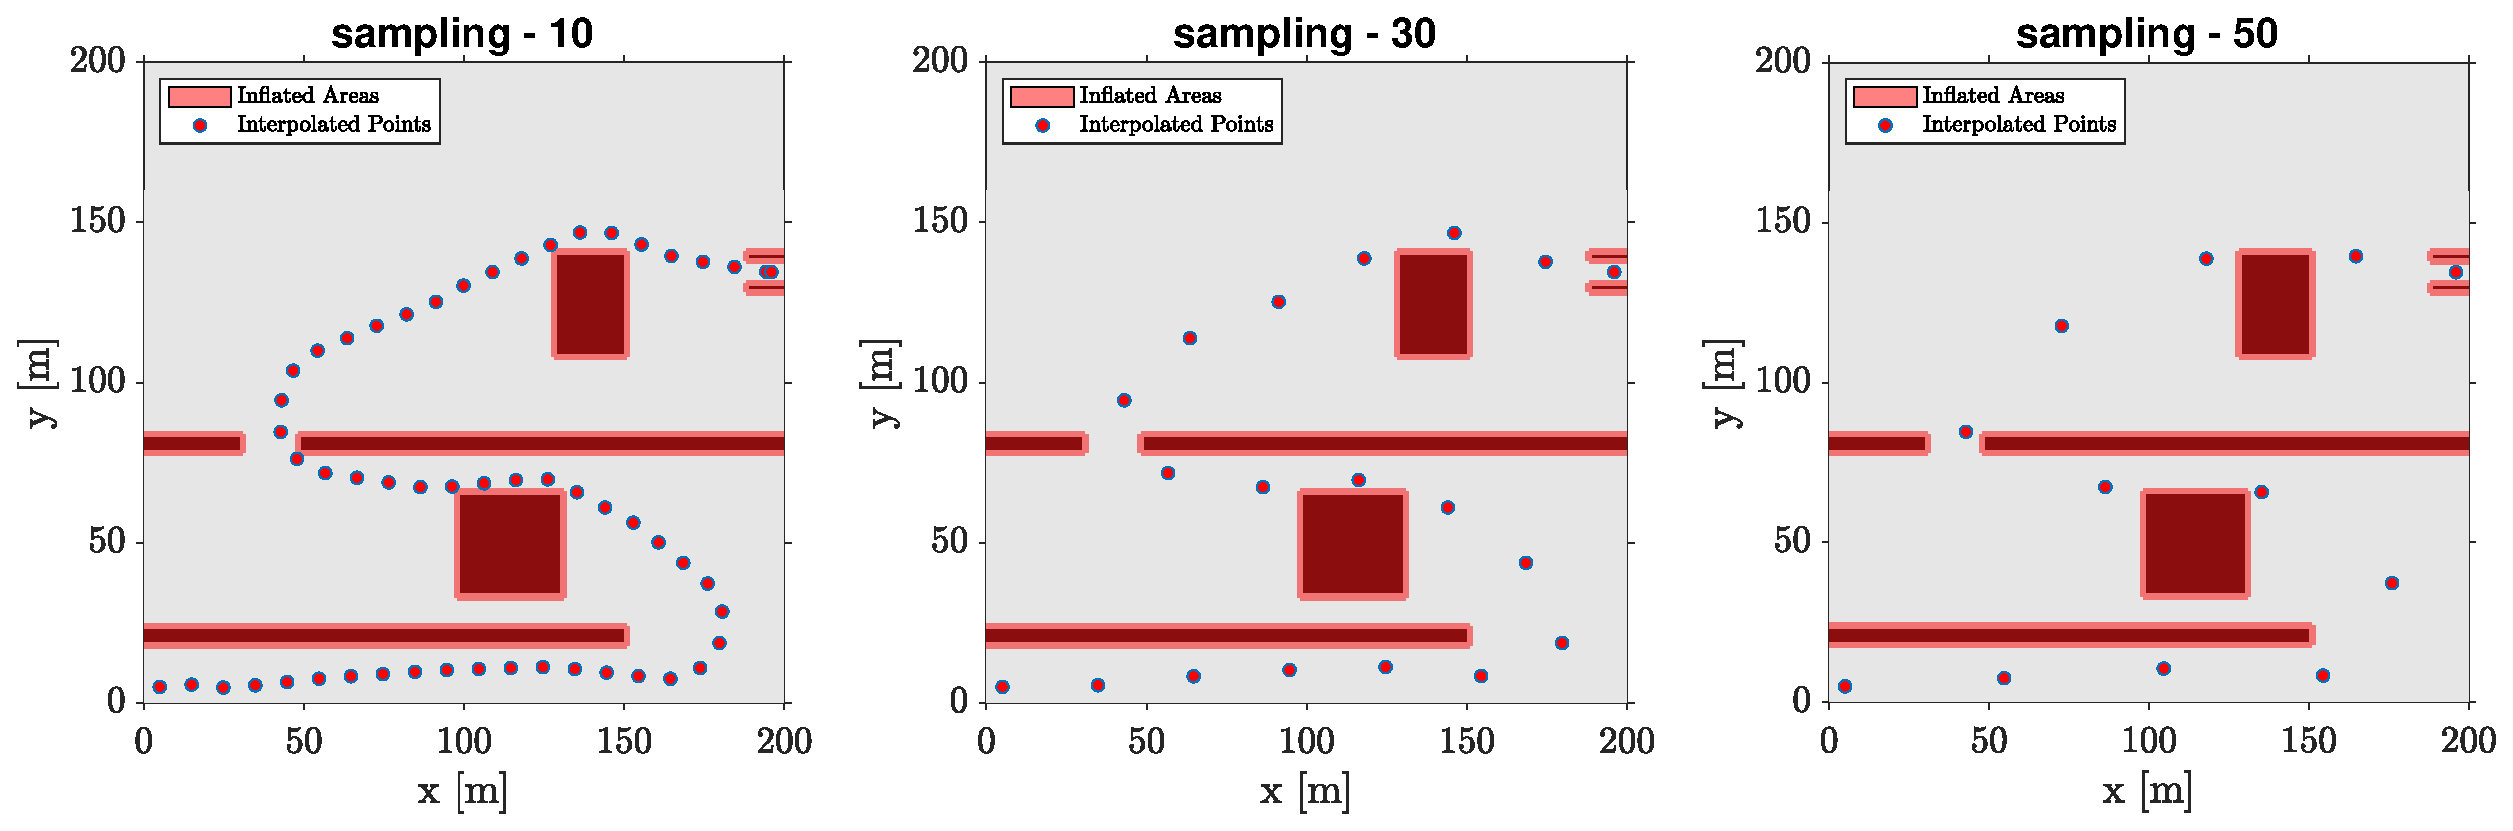
\includegraphics[width=0.99\linewidth]{ex7/q1/ex-71samp1.eps}
        \centering
        \caption{Effect of interpolation samples parameter on path resolution}
        \label{71samp1}
        \end{figure}

Using the clothoid based lateral controller, the interpolated path for each interpolation sample was tested, and the results are shown in Figure \ref{71samp2}. The tracked path becomes smoother with higher interpolation sample number, which makes it easier to stabilize the vehicle. This is evident in the tracking error results [Figure \ref{71samp3}].

        \begin{figure}[ht]
        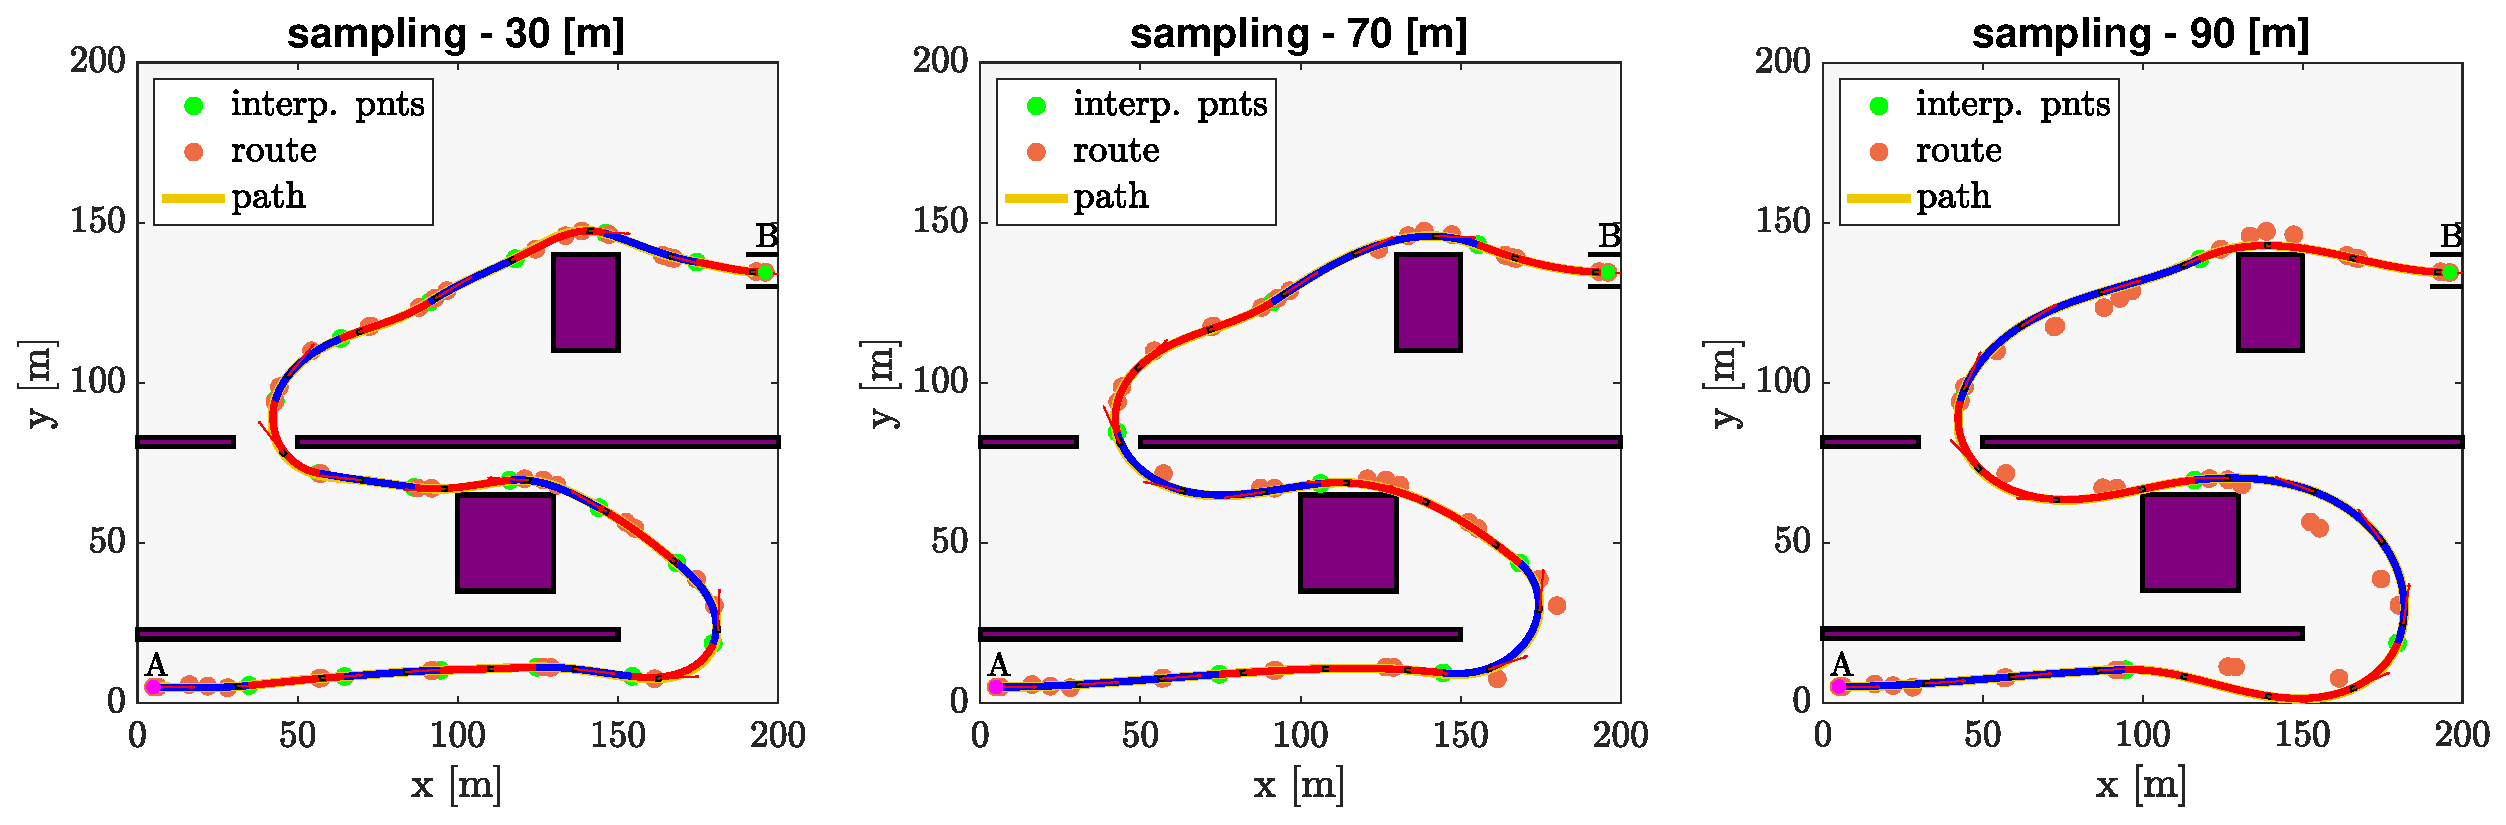
\includegraphics[width=0.99\linewidth]{ex7/q1/ex-71samp2.eps}
        \centering
        \caption{Clothoid based controller tracking different interpolation samples}
        \label{71samp2}
        \end{figure}

The interpolation sample is a very useful tool to apply. As demonstrated, it smooths out the generated path making it easier for the controller to track it. An ideal interpolation sample for our test would be 50 or 70.\newpage

        \begin{figure}[ht]
        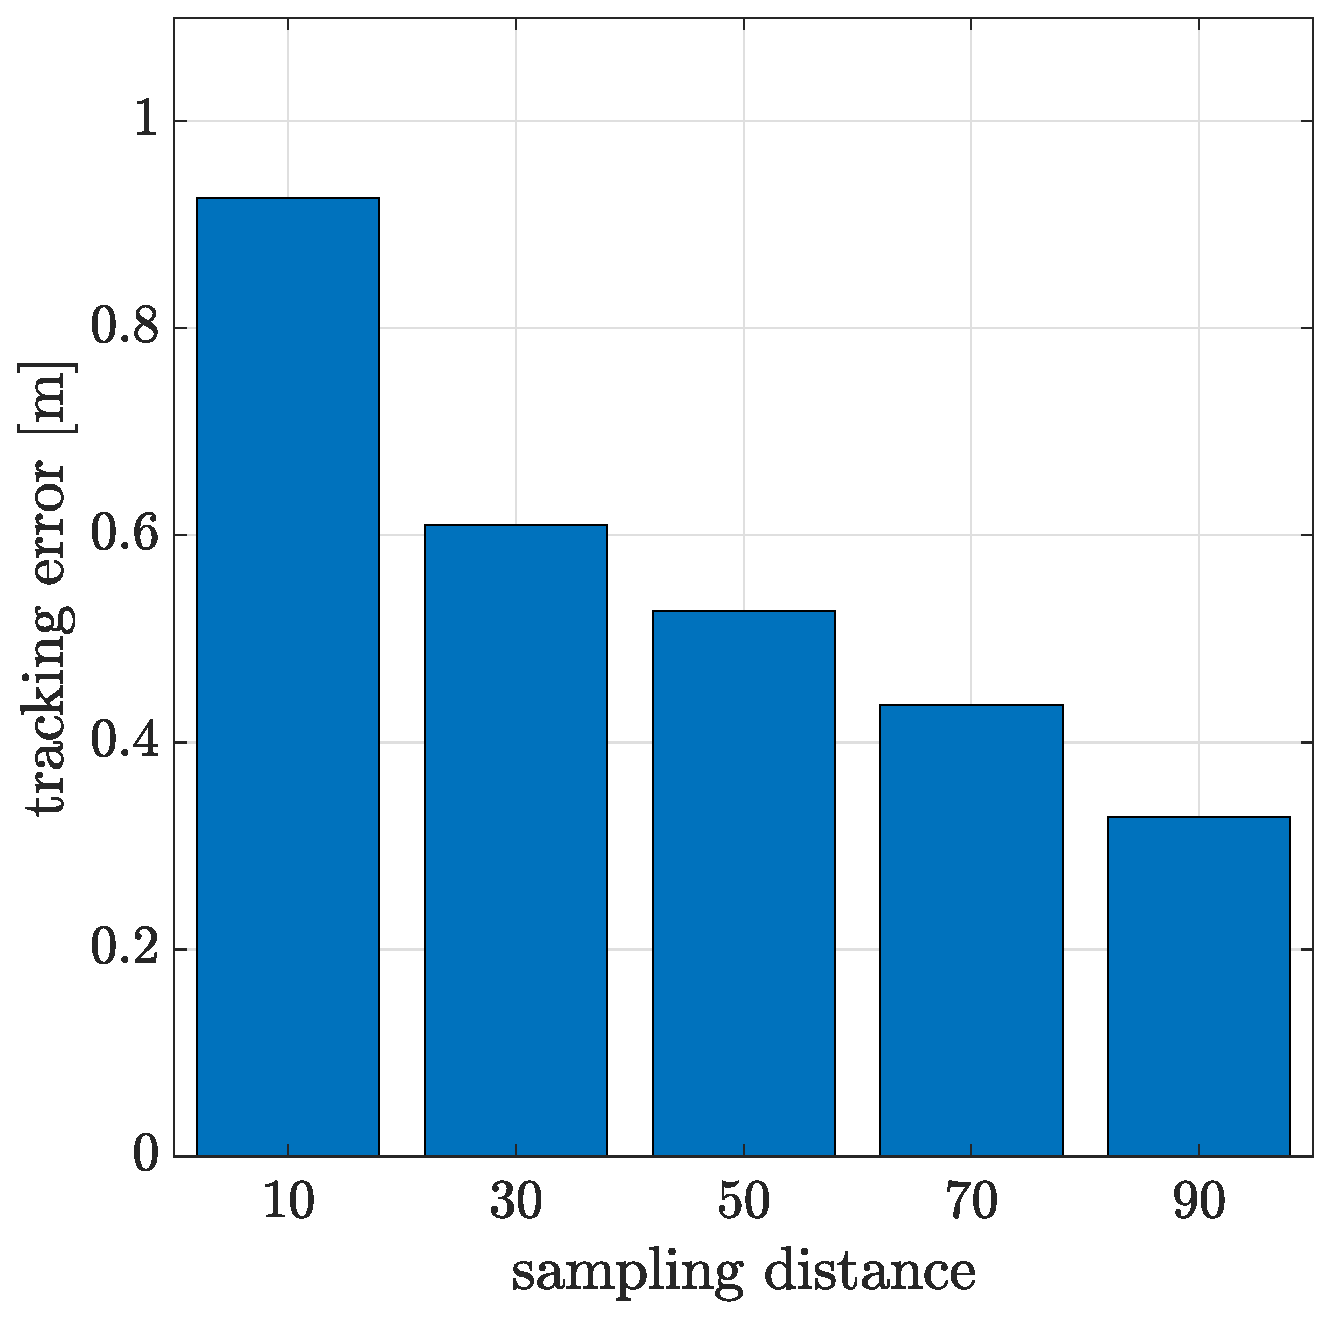
\includegraphics[width=0.6\linewidth]{ex7/q1/ex-71samp3.eps}
        \centering
        \caption{Tracking error at 50 km/h with different interpolation sample}
        \label{71samp3}
        \end{figure}

Clothoid fitting of the path is better than Dubins path because of the following reasons:
\begin{itemize}
\item Dubins path is only limited to three different maneuvers[straight, left or right turns] in six different combinations [RSR, LSL, RSL, LSR, RLR, and LRL].
\item All the turns of the Dubins path only have a fixed radius of curvature.
\end{itemize}

Given the results achieved with the optimized RRT*, it is evident that it is a robust and efficient algorithm. It was able to find a feasible and a nearly optimal solution within seconds [Table \ref{tab:7.1}]. The route quality was mostly smooth, however, that could be remedied with clothoid fitting and sample interpolation as was demonstrated in Figure \ref{71samp2}. Furthermore, RRT* is capable of taking into account the dynamics of the vehicle, however, that could impact it's computational time performance. As a conclusion, RRT* is very well suited for a high level planning algorithm.

During the tracking tests conducted, the vehicle starts and maintains the same speed, until it reaches the parking lot, where it decelerates to 20 km/h. I implemented a simulation auto stopping feature to terminate once the vehicle reaches target destination within a threshold. In addition, the look ahead starts receding once the remaining distance is smaller than the look ahead value.

A route was generated using [c\_dist = 45, itr = $10^{4}$, $\delta$ = 5$^\circ$], then tested with the clothoid based lateral controller at $u$ = [30, 50, 70]. The results of the test are shown in Figure \ref{71vpt}.
        \begin{figure}[ht]
        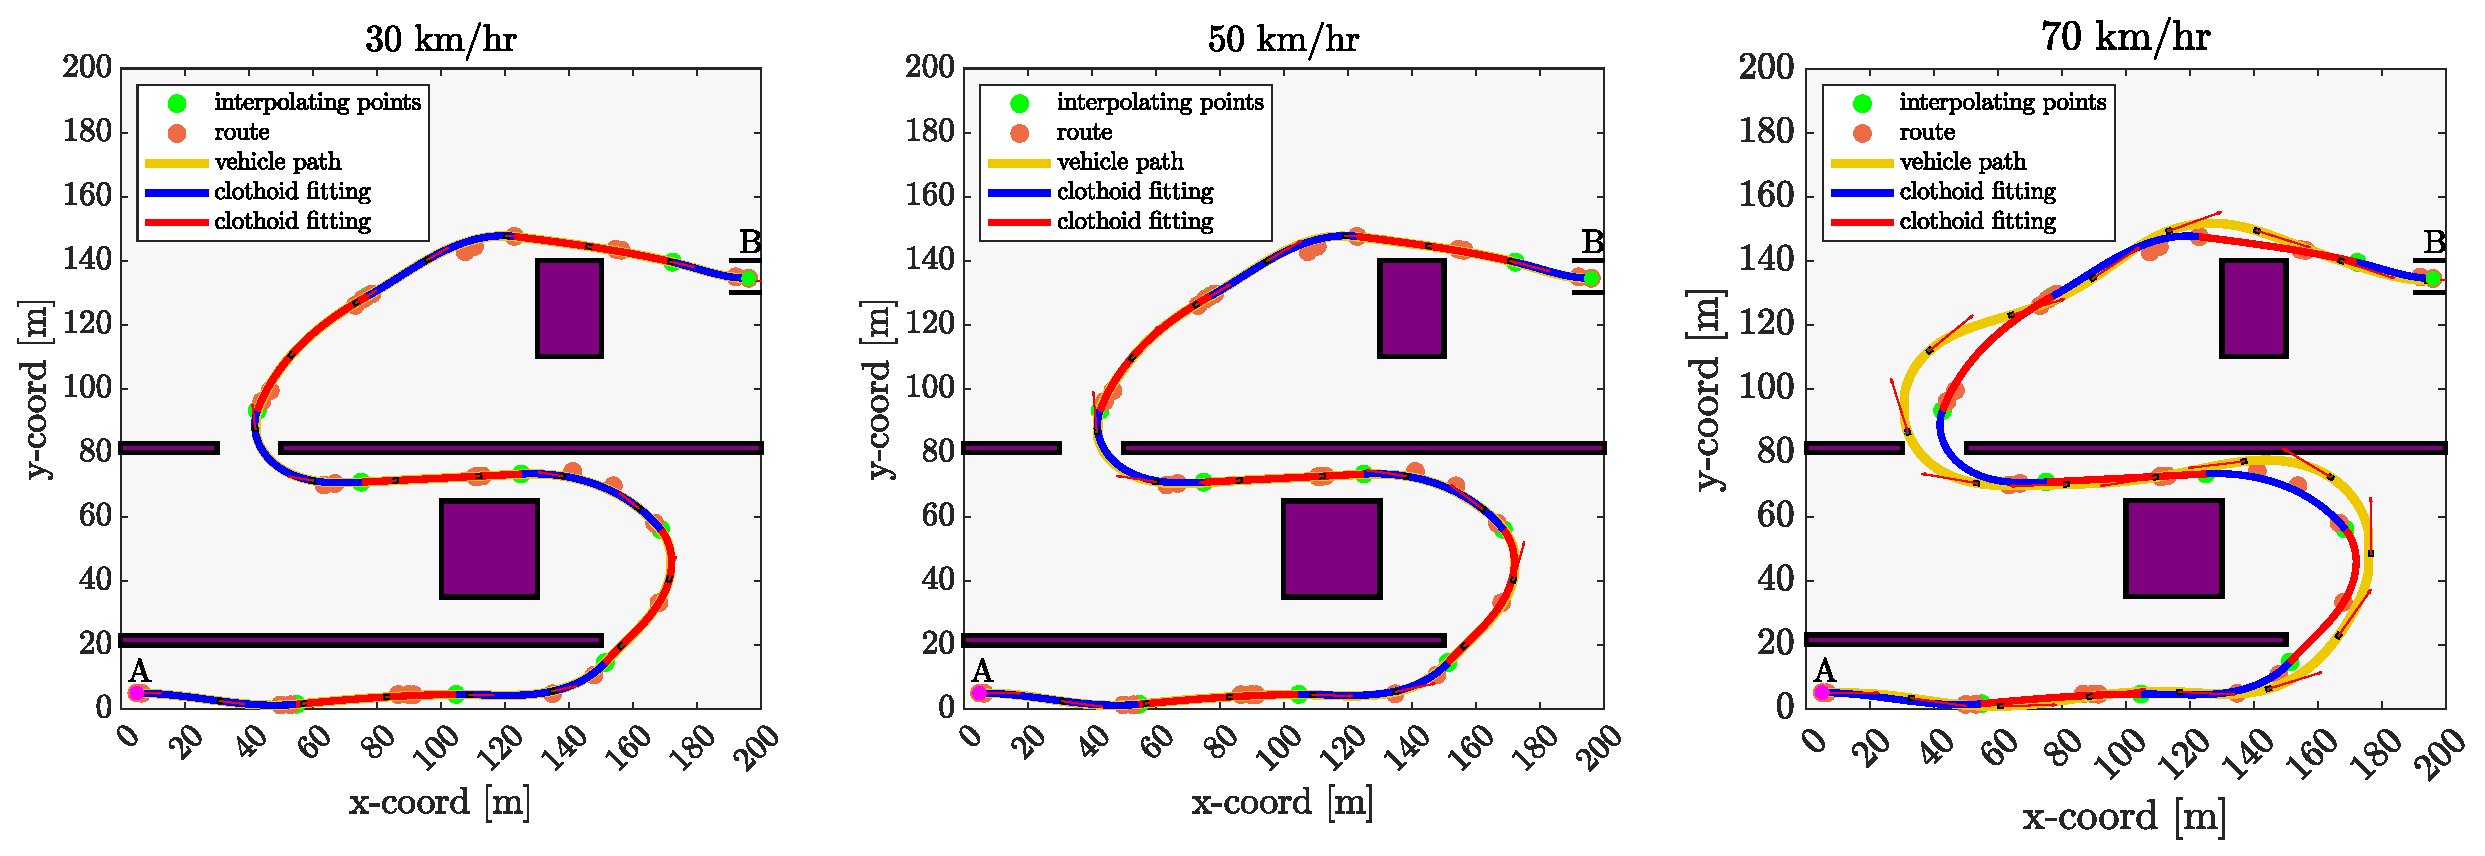
\includegraphics[width=0.99\linewidth]{ex7/q1/ex-71vpt.eps}
        \centering
        \caption{Clothoid based lateral controller tracking RRT* result at different speeds}
        \label{71vpt}
        \end{figure}

The vehicle tracking worked well with $u$ = [30, 50] km/h. However, tracking error rose significantly at 70 km/h [results are in Figure \ref{71et4}]. Summarized results are in Table \ref{tab:7.2}.

        \begin{figure}[ht]
        \includegraphics[width=0.5\linewidth]{ex7/q1/ex-71et-4.eps}
        \centering
        \caption{Tracking error for clothoid based lateral controller tracking RRT* path}
        \label{71et4}
        \end{figure}



\begin{table}[ht]
    \centering
    \begin{tabular}{c | c | c | c }
      \textbf{$u$ [km/h]}  & \textbf{tracking time [s]} & \textbf{tracking error [m]} & \textbf{route calculation time [s]} \\ \hline
\multicolumn{1}{c|}{30} & \multicolumn{1}{c|}{62.4} & \multicolumn{1}{c|}{0.2} &\multicolumn{1}{l}{} \\\cline{1-3}
\multicolumn{1}{c|}{50} & \multicolumn{1}{c|}{37.5} & \multicolumn{1}{c|}{0.6} &\multicolumn{1}{c}{1.6} \\\cline{1-3}
 \multicolumn{1}{c|}{70} & \multicolumn{1}{c|}{28.8} & \multicolumn{1}{c|}{13.6} &\multicolumn{1}{l}{} 

    \end{tabular}
    \caption{Route calculation and tracking performance comparison}
    \label{tab:7.2}
\end{table}

The time required to calculate the route using RRT* is much shorter than how long it takes to travel the path. This means RRT* can be used in this application to calculate the route online.

The biggest bottleneck for traveling time is certainly the speed at which the car is moving. The higher the speed, the shorter the travel time as shown in Table \ref{tab:7.2}. However, the controller's capability falls short at higher speeds causing a major unsafe tracking error.

RRT* could be be contributing to the bottleneck if the generated path requires higher steering input. The clothoid fitting alleviates the issue by smoothing out the route and allowing the vehicle to travel faster through turns.

\section{Exercise 2 - lateral control}


The lateral controllers tested earlier will be used on the path that RRT* has generated offline. The controllers will be compared to each other in terms of performance in tracking error, tracking time, and steering behaviour. The list of lateral controllers are as follows:
\begin{itemize}
    \item Clothoid based lateral control
    \item Pure pursuit
    \item Stanley kinematic
    \item Stanley dynamic
\end{itemize}

The controllers have already been optimized in the previous chapter and the best resulting parameters are going to be utilized in the following tests.

RRT* generated a reference path offline, and each controller used said reference path for tracking at u = [30, 50, 60] km/h. Results of the tracking error is displayed in Figure \ref{72er}. 
        \begin{figure}[ht]
        \includegraphics[width=0.6\linewidth]{ex7/q2/ex-72er.eps}
        \centering
        \caption{Tracking error for lateral controllers following RRT* path}
        \label{72er}
        \end{figure}

        \begin{figure}[ht!]
        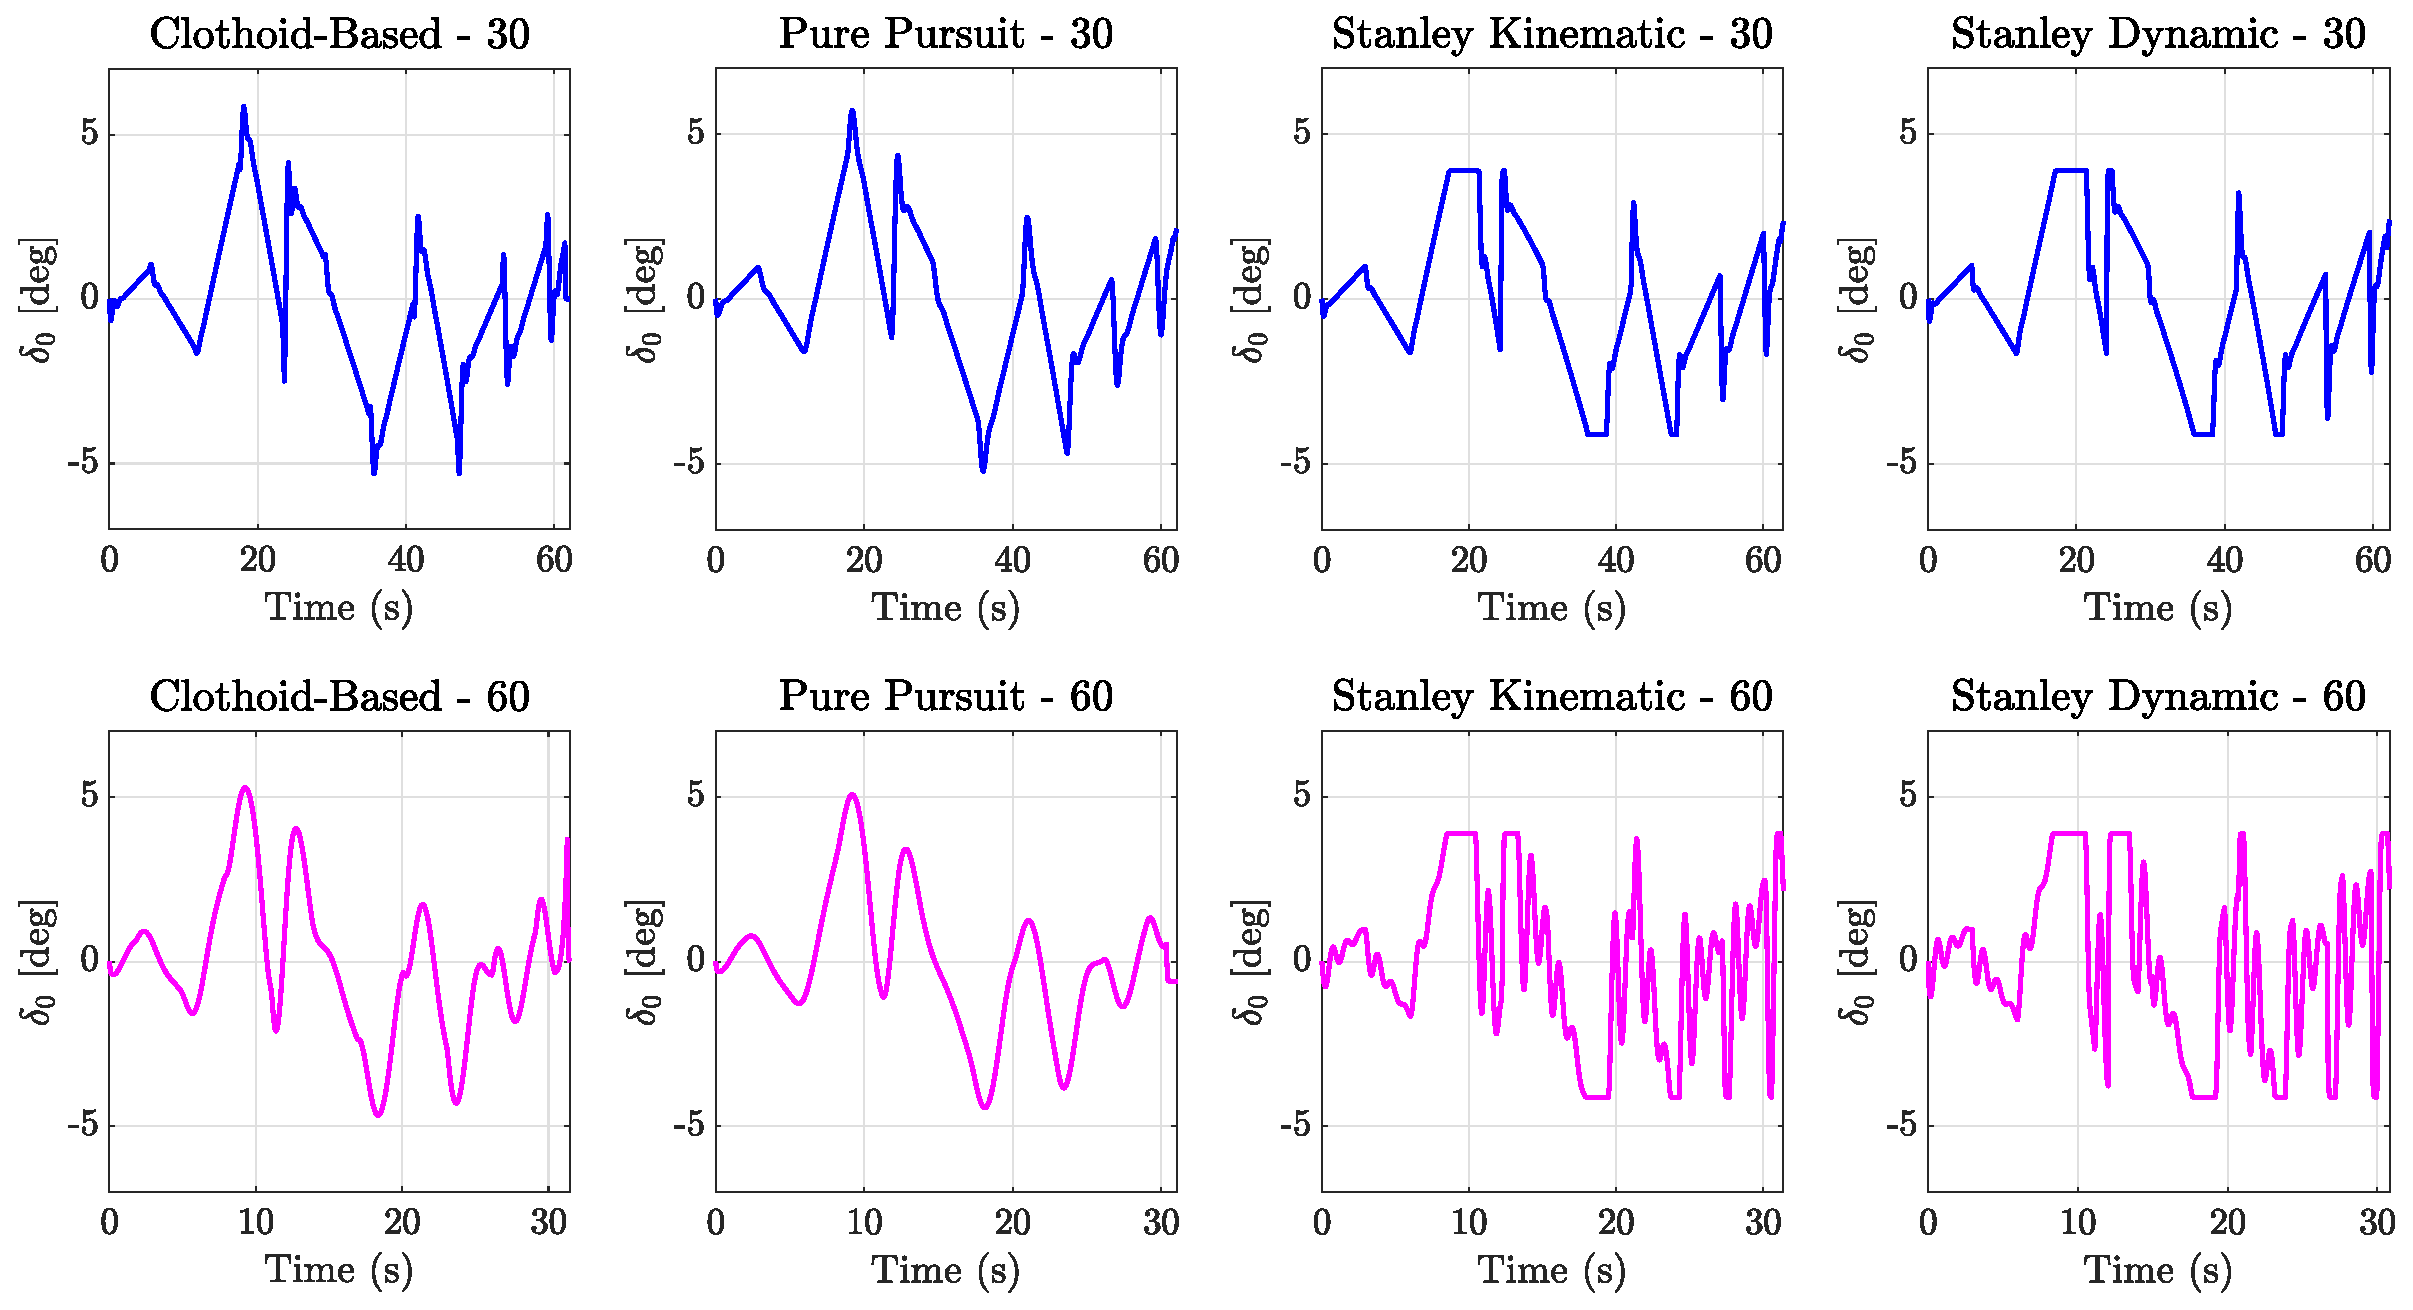
\includegraphics[width=0.99\linewidth]{ex7/q2/ex-72ff.eps}
        \centering
        \caption{lateral controllers steering behaviour following RRT* path}
        \label{72ff}
        \end{figure}

The tests agreed with the previous results achieved in the last chapter. From a tracking error metric prospective, both clothoid based and pure pursuit controllers did well in low speed. However, pure pursuit is much better in higher speeds compared to the rest. Stanley Kinematic struggled on both low and high speeds with the highest tracking error.

Figure \ref{72ff} is the steering behaviour for all the controllers at each speed. The pattern profile for the controllers looked very similar at low speed. Both of the Stanley controllers have a cut off because their max steer parameter is set at 4$^\circ$.

At the higher speed, pure pursuit seemed to perform the best showing smoother curves. The Stanley controllers struggled and exhibited a lot of oscillations and jitters. The results for the tests are all summarized in table \ref{tab:7.3}. The green colored cells highlight the best performer in each category for both speeds.

\begin{table}[ht!]
    \centering
    \begin{tabular}{c|c|c|c|c|c|c} 
       \multirow{3}{*}{\textbf{Controller}} & \multicolumn{3}{c|}{\textbf{$u$ = 30 km/h}} & \multicolumn{3}{c}{\textbf{$u$ = 60 km/h}} \\
        \cline{2-7}

 & \multirow{2}{1.3cm}{\centering\textbf{time [s]}} & \multirow{2}{1.3cm}{\centering\textbf{error [m]}} & \multirow{2}{2.2cm}{\centering\textbf{total steer input [$^\circ$]}}
& \multirow{2}{1.3cm}{\centering\textbf{time [s]}} & \multirow{2}{1.3cm}{\centering\textbf{error [m]}} & \multirow{2}{2.2cm}{\centering\textbf{total steer input [$^\circ$]}}\\
 &&&&&&\\\hline

         Clothoid-based  & \cellcolor{green!10}62.0 &  0.12 & 82.6 & 31.4 & 2.20 & 67.2 \\ \hline
        
        Pure pursuit & 62.1 &  \cellcolor{green!10}0.07 & 68.6 & 31.0 & \cellcolor{green!10}1.42 & \cellcolor{green!10}49.1\\ \hline
        
        S. kinematic & 62.7 &  3.40 & \cellcolor{green!10}66.7 & 31.3 & 5.09 & 142.9 \\ \hline
        
        S. dynamic & 62.2 &  2.52 & 71.7 & \cellcolor{green!10}30.8 & 3.59 & 151.9 \\ 
    \end{tabular}
  \caption{Comparison of lateral controllers results}
  \label{tab:7.3}
\end{table}

The time taken to get to target is almost identical between the controllers because the bottleneck is the speed of the car. For the tracking error metric, pure pursuit performed best at both low and high speeds.

To put a metric on the steering behaviour, I calculated the total steering input for each run in degrees [results are in Table \ref{tab:7.3}]. It was computed by summing the absolute values of the change in steering angle between every two consecutive time steps [equation \ref{eq:7.1}].

\begin{equation}\label{eq:7.1} 
 \delta_{tot} = \sum_{n=1}^{N} |\delta_{i} - \delta_{i+1}|
\end{equation}

Results agreed with the visual graphs in Figure \ref{72ff}, which suggests that pure pursuit had the least amount of total steer input for both low and high speeds, with clothoid based being the second best. A list of the pros and cons for each controller are included in Table \ref{tab:6.5}.